\documentclass[tikz,border=5mm]{standalone}
\usetikzlibrary{decorations.markings}

\begin{document}
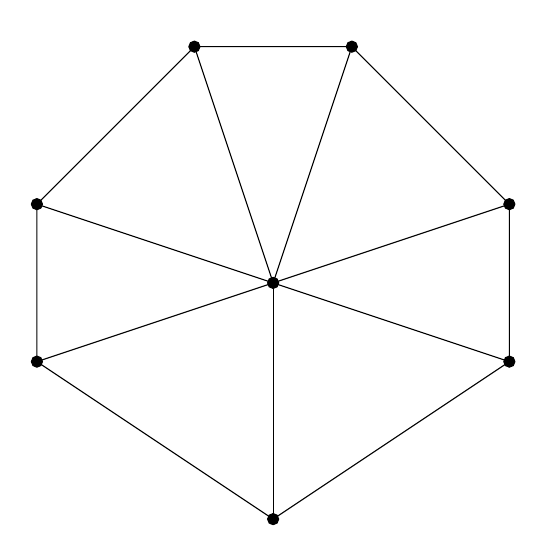
\begin{tikzpicture}[every loop/.style={min distance=30mm}]

    % these are the vertices
    \draw[fill=black] (10,10) circle (2pt) node[above] {};
    \draw[fill=black] (12,10) circle (2pt) node[above] {};
    \draw[fill=black] (8,8) circle (2pt) node[above] {};
    \draw[fill=black] (14,8) circle (2pt) node[above] {};
    \draw[fill=black] (8,6) circle (2pt) node[above] {};
    \draw[fill=black] (14,6) circle (2pt) node[above] {};
    \draw[fill=black] (11,4) circle (2pt) node[above] {};
    \draw[fill=black] (11,7) circle (2pt) node[above] {};

    \draw (10,10) -- (12,10) -- (14,8) -- (14,6) -- (11,4) -- (8,6) -- (8,8) -- (10,10);
    \draw (10,10) -- (11,7) -- (12,10);
    \draw (8,8) -- (11,7) -- (14,8);
    \draw (8,6) -- (11,7) -- (14,6);
    \draw (11,4) -- (11,7);

\end{tikzpicture}
\end{document}
